\documentclass[a4paper,twoside,final]{article}
%----Eingebundene Bibliotheken-----
\usepackage[ngerman]{babel}         % Deutsches Sprachpaket
\usepackage[utf8]{inputenc}         % Eingaben codieren
\usepackage[T1]{fontenc}            % Umlaute codieren, Silbentrennung
\usepackage{amsmath, amssymb}       % Mathe
\usepackage{amsthm,amstext,amsxtra} % Symbole für Mathe
\usepackage{mathtools}              % \Aboxed Boxen in align
\usepackage{wrapfig}                % Bilder umfließen
\usepackage{svg}                    % Vektorgraphiken einbinden
\usepackage{geometry}               % Papierformat
\usepackage{tabularx}               % Tabellen
\usepackage{xcolor,colortbl}        % Farben
\usepackage{graphicx}               % Für Limes Definition wichtig
\usepackage{soul}                   % Unterstreichungen
\usepackage[section]{placeins}      % \Floatbarrier
\usepackage{wrapfig}                % Bilder umfließen
\usepackage{enumerate}              % Aufzählungen
\usepackage{footnote}               % Fußzeilen
\usepackage{booktabs}               % publication quality tables
\usepackage[hyphens]{url}           % \url{}
\usepackage{bm}                     % bold symbols \bm{r}
\usepackage{dsfont}                 % identity matrix \mathds{1}
\usepackage{enumitem}               % itemize Umgebungen customizen
\usepackage{esint}                  % Doppelintegrale
\usepackage{fancyhdr}               % schöne Kopf- und Fußzeilen
\usepackage{lmodern}
\usepackage{tikz}
\usepackage{pgfmath, pgfplots}
\usepackage[labelfont=bf]{subcaption}
\usepackage[square,numbers,sort&compress]{natbib}
\usepackage{mhchem}                 % Chemistry Package
\usepackage{physics}
\usepackage{chemfig}
\usepackage[detect-all,
            locale=DE,binary-units,
            exponent-product=\cdot
            ]{siunitx}              % \SI{12}{\gram}
%siunitx stellt für Tabellen den Spaltentyp S bereit ==> Ausrichtung an Dezimaltrennzeichen
\usepackage[position=below,
            tableposition=top,
            format=hang,
            labelfont=it,
            labelfont=bf,
            ]{caption}              % Settings für Captions
\captionsetup[wrapfigure]{name=Abb.}
\usepackage[europeanvoltages,
            europeancurrents,
            europeanresistors,
            americaninductors,
            europeanports
            ]{circuitikz}           % Schaltungen
\usepackage{chngcntr}               % vor hyperref laden!
  \counterwithin*{equation}{section}
  \counterwithin*{figure}{section}
  \counterwithin*{table}{section}

\usepackage[final,
            pdfauthor={Martin Beyer, Vanessa Huth},
            pdfsubject={Fortgeschrittenen-Praktikum},
            pdffitwindow=true,      % resize document window
            pdftitle={Fortgeschrittenen-Praktikum},
            bookmarks=true,         % lesezeichen-Liste
            bookmarksopen=true,     % Lesezeichen geöffnet
            bookmarksopenlevel=1,
            bookmarksnumbered=true,
            colorlinks=true,        % fuer Druckversion auf "false"
            linkcolor=blue,         % Table of Contents, Footnotes
            urlcolor=blue,          % fuer eingebunden URLs
            citecolor=blue,         % Equations, References
            filecolor=blue,
            pdfborder={0 0 0},      % keine Rahmen um Links: {0 0 0}
            ]{hyperref}


% Commands
\renewcommand{\sfdefault}{lmss}     % latin modern sans serif
\newcommand{\R}{\mathbb{R}}         % Reelle Zahlen
\newcommand{\N}{\mathbb{N}}         % Natürliche Zahlen
\newcommand{\C}{\mathbb{C}}         % Komplexe Zahlen
\newcommand{\de}{\mathrm{d}}      % Differential
\newcommand{\entspricht}{\mathrel{\widehat{=}}}

\DeclareSIUnit{\eV}{\text{eV}}
\DeclareSIUnit{\voltpeakpeak}{\volt{\textsubscript{pp}}}

% Dokumenteneinstellungen
\setlength{\parindent}{0px}         % remove indent in new paragraph
\setlength{\parindent}{0px}         % keine Absätze durch Leerzeilen im Code
\emergencystretch=1em % Definiert den Leerraum, der innerhalb einer Zeile zusätzlich verteilt werden darf.
\setlength{\topmargin}{-5mm} % 210mm = 8.2677165in
\newlength{\mylength}
\setlength{\mylength}{\paperwidth}
\addtolength{\mylength}{-2in} % standardmäßig wird den Seitenrändern jeweils noch 1in = 25.4mm hinzuaddiert
\setlength{\textwidth}{145mm}
\setlength{\textheight}{230mm}
\addtolength{\mylength}{-\textwidth}
\setlength{\oddsidemargin}{10mm}
\addtolength{\mylength}{-\oddsidemargin}
\setlength{\evensidemargin}{\mylength}
\setlength{\marginparwidth}{1.7cm}
\interfootnotelinepenalty=10000

% Umdefinition von \textcolor ********************************************************
\makeatletter
\renewcommand*{\@textcolor}[3]{%
	\protect\leavevmode
	\begingroup
	\color#1{#2}#3%
	\endgroup
}
\makeatother
% Damit das auch im Mathemodus anwendbar ist und dort z.B. die Leerzeichen nicht wie im Textmodus gesetzt werden.

\pgfplotsset
{compat=newest, % aktuelle Version: 1.16 [29.05.2018]
	/pgf/number format/.cd, % cd steht fuer current directory
	%  	use comma, % Komma als Dezimaltrennzeichen %%% UNCOMMENT THIS !!!
	1000 sep={} % Legt das Tausendertrennzeichen fest
}
%\usepgfplotslibrary{external} % Section 7.1.1 Using the Automatic Externalization Framework of TikZ
%\tikzexternalize[prefix=FiguresTikZ/] % activate externalization! Use subdirectory [FiguresTikZ]
\usepgfplotslibrary{fillbetween}
\usepgfplotslibrary{polar}
\usetikzlibrary{arrows.meta}
\usetikzlibrary{calc}
\usetikzlibrary{datavisualization.formats.functions}
\usetikzlibrary{intersections}
\usetikzlibrary{patterns}
\usetikzlibrary{pgfplots.colormaps}
\usetikzlibrary{plotmarks}
\usetikzlibrary{shapes.geometric}

% Generelle Festlegung des Styles fuer Blockschemata (Plaene fuer Regelkreise, etc.)
\tikzstyle{block} = [draw, fill=blue!20, rectangle, minimum height=1cm, minimum width=1cm]%, minimum width=6em]
\tikzstyle{sum} = [draw, fill=blue!20, circle, node distance=1cm]
\tikzstyle{input} = [coordinate]
\tikzstyle{output} = [coordinate]
\tikzstyle{pinstyle} = [pin edge={to-,thin,black}]

\begin{document}
\setlength{\marginparsep}{2em}
\renewcommand{\theequation}{\arabic{section}.\arabic{equation}}
\renewcommand{\thefigure}{\arabic{section}.\arabic{figure}}
\renewcommand{\thetable}{\arabic{section}.\arabic{table}}

% Anfang ********************************************************
\begin{center}
\thispagestyle{empty}
  
\includegraphics[width=0.75\textwidth]{UniJena_BildWortMarke_black.pdf}\\[4em]
  \Large
  Ausarbeitung zum Versuch\\[2em]
  \Huge
  Debye-Sherrer-Verfahren\\
  \vspace{2cm}
  \Large
  Martin Beyer und Vanessa Huth\\[2em]
  Abgabe: 05. November 2019\\[2em]
  Betreuer: Dr. Uschmann\\[5em]
  \begin{flushleft}
  	Bewertung und Ausarbeitung:\\[2em]
		Protokollführung und Form:\\[1em]
		Ergebnisse, Auswertung und Interpretation:\\[1em]
		Bemerkungen und Hinweise des Betreuers:
  \end{flushleft}
\end{center}
\clearpage

\pagestyle{fancy}
\renewcommand{\headrulewidth}{0pt}
\renewcommand{\footrulewidth}{0.5pt}
\renewcommand{\sectionmark}[1]{\markright{#1}}
\fancyhead[RO,LE]{\textbf{Debye-Sherrer-Verfahren}}
\fancyhead[RE,LO]{\rightmark}
\fancyfoot[LE,RO]{\bfseries\thepage}
\fancyfoot[CO,CE]{Protokoll}
\renewcommand{\headrulewidth}{0.5pt}
\renewcommand{\footrulewidth}{0.5pt}

\setcounter{equation}{0}
\setcounter{figure}{0}

% *********************************************
% ***** KAPITEL 1 *****************************
% *********************************************

\section{Aufgabenstellung} \label{sec:Aufgabenstellung}
\paragraph{Aufgabe 1}$~$\\
 Es sollen zwei Diffraktogramme einer polykristallinen kubischen Substanz mit einer Debye\--Scherrer\--Ka\-me\-ra aufgenommen werden, einmal ohne und einmal mit einem geeigneten Absorptionsfilter für die Röntgenspektrallinien von Kupfer. Anschließend sind die Debye-Sherrer-Ringe beider Aufnahmen den K$\alpha$- und K$\beta$- Linien zuzuordnen. Durch Zuordnung der Gitterkonstanten soll die untersuchte Substanz identifiziert werden. Dafür müssen die Reflexe indiziert, systematische Auslöschungen benannt und eine ausführliche Fehlerdiskussion der Gitterkonstanten unter Verwendung eines geeigneten Extrapolationsverfahrens durchgeführt werden.
\paragraph{Aufgabe 2}$~$\\
Die maximale Probenabsorption soll unter Annahme der Festkörperdichte für die Probe berechnet werden. Bei der Benutzung einer Glaskapillare als Probenhalter soll auch deren Absorption für die verwendete charakteristische Strahlung berechnet werden. Anschließend ist das Ergebnis im Zusammenhang mit den Ergebnissen aus Aufgabe 1 zu diskutieren.
\paragraph{Aufgabe 3}$~$\\
Eine Berechnung der Reflexintensitäten soll durchgeführt und mit den aus der Filmtransmission ermittelteten Intensitätsverhältnissen verglichen werden.
\paragraph{Aufgabe 4}$~$\\
Das getestete Röntgen-Analyse-Verfahren nach Debye und Scherrer (als nicht nur rein \glqq historische\grqq{} Methode der Pulverdiffraktometrie) soll gewertet werden..


% *********************************************
% ***** KAPITEL 2 *****************************
% *********************************************
\section{Grundlagen} \label{sec:Grundlagen}

\subsection{Röntgenstrahlung}
Röntgenstrahlen wurden 1895 von \textsc{Wilhelm Conrad Röntgen} entdeckt und stellen einen Teil des elektromagnetischen Spektrums im Bereich von $\lambda = \SI{5}{\pico \metre}\hdots \SI{1}{\nano\metre}$ dar. Sie zeichnen sich durch ihre hohe Photonenenergie und ein großes Durchdringungsvermögen aus. Die hohe Durchdringungsrate lässt sich zur zerstörungsfreien Untersuchung von Stoffen verwenden. Bei der im Versuch verwendeten Methode handelt es sich um eine Feinstrukturuntersuchung, wo beim Durchgang der Röntgenstrahlen durch kristalline Substanzen charakteristische Beugungserscheinungen zu beobachten sind.\\
Da die Brechzahl in allen Materialien im Röntgenbereich sich kaum von 1 unterscheidet, lassen sich keine optischen Bauelemente wie Prismen oder Linsen verwenden. Stattdessen wird die \textsc{Bragg}reflexion an ebenen Kristallen genutzt.\\
Die Röntgenstrahlung in diesem Versuch wird durch eine Röntgenröhre erzeugt, wo in einem evakuierten Raum mithilfe hoher Spannungen an einer Kathode Elektronen herausgelöst und fokussiert und auf auf eine Anode beschleunigt werden.
\begin{figure}[htp]
    \centering
    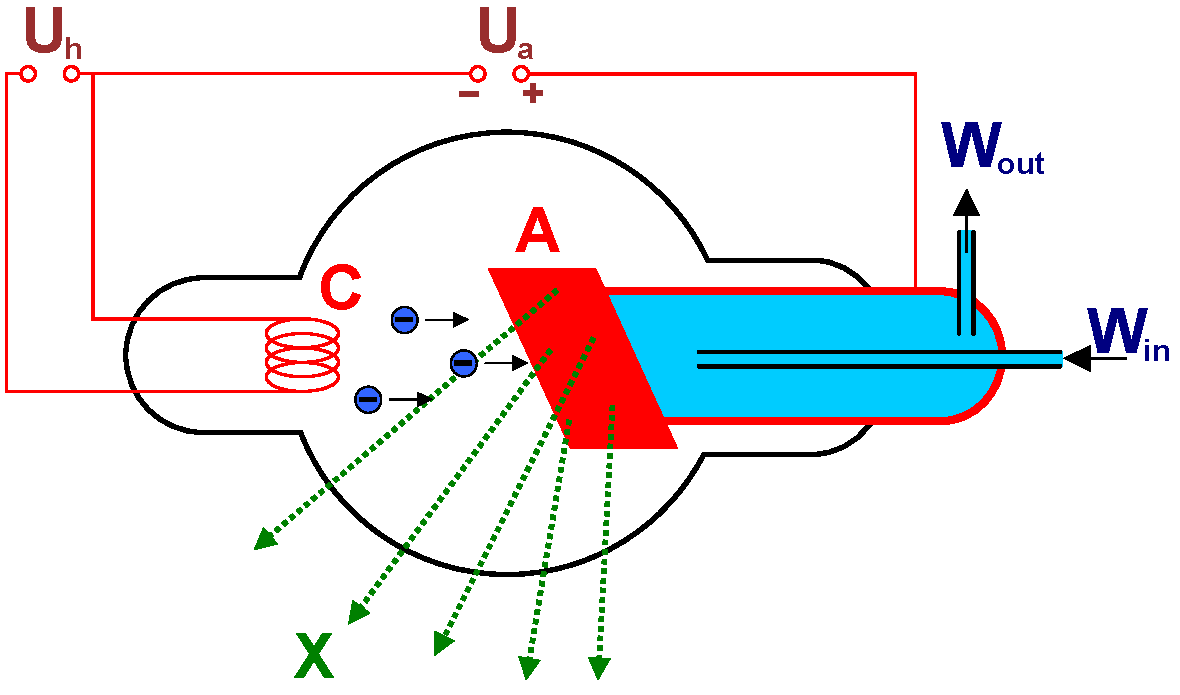
\includegraphics[width=0.5\textwidth]{Abbildungen/WaterCooledXrayTube.pdf}
    \caption{Schematischer Aufbau einer Röntgenröhre nach~\cite{Roentgenroehre}. Da beim Aufprall der Elektronen viel Wärme entsteht, muss die Anode mithilfe eines Wasserzuflusses $W_\text{in}$ gekühlt werden.}
    \label{fig:Roentgenroehre}
\end{figure}\\
Beim Aufschlagen auf die Anode werden die Elektronen abgebremst und strahlen Energie in Form von elektromagnetischen Wellen ab. Idealerweise würde die gesamte kinetische Energie in Röntgenstrahlung umgewandelt werden.
\begin{align}
  e U = E_\text{kin} = h \cdot \nu_\text{max} = \frac{hc}{\lambda_\text{min}}
\end{align}
Allerdings wird ein großer Teil der kinetischen Energie in Wärme umgesetzt, sodass die Anode gekühlt werden muss. Der schematische Aufbau einer Röntgenröhre ist in Abbildung~\ref{fig:Roentgenroehre} dargestellt.\\
Das Emissionsspektrum der Anode wird durch ihr Material und der Beschleunigungsspannung der Röntgenröhre bestimmt und setzt sich aus zwei Komponenten zusammen.\\
Die erste Komponente wird \glqq{}weiße Röntgenstrahlung\grqq{} genannt und erscheint allein durch das Abbremsen der Elektronen in der Oberflächenschicht des Targets. Die zweite Komponente bildet die charakteristische Röntgenstrahlung, die normalerweise aus zwei Linien besteht. Hier geschehen Übergänge zwischen den inneren Schalen der Atome des Targets. Gewöhnlich sind die Schalen vollständig mit Elektronen besetzt, jedoch können die hochenergetischen, eingeschossenen Elektronen die gebundenen Elektronen herausschlagen und dort freie Energieniveaus erzeugen. In diese können anschließend Elektronen höherer Niveaus unter Photonenemission übergehen. Diese Linien fester Frequenz werden im Spektrum als K$_\alpha$- bzw. als K$_\beta$-Linien bezeichnet (siehe Abbildung~\ref{fig:Roentgenspektrum}). Das 'K' steht für die Schale, die besetzt wird und der Index beschreibt, aus welcher Schale das Elektron kam, welches den Platz besetzt. Für $\alpha$ handelt es sich um die nächstliegende L-Schale.\vspace{-5mm}
\begin{figure}[htp]
    \centering
    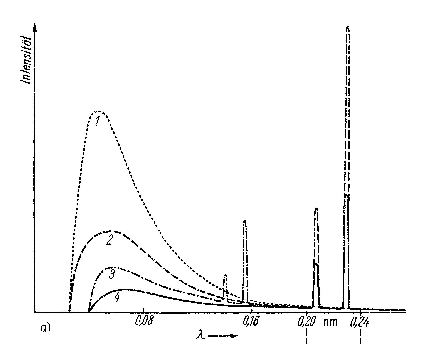
\includegraphics[width=0.5\textwidth]{Abbildungen/Roentgenspektrum.pdf}
    \caption{Brems- und charakteristisches Spektrum von Röntgenröhren mit verschiedenem Anodenmaterial. Bei der größten Emissionslinie handelt es sich um die K$_\alpha$-Linien. Bei $\lambda =\SI{0,21}{\nano\metre}$ befinden sich die K$_\beta$-Linien.~\cite[S.361]{Kleber}}
    \label{fig:Roentgenspektrum}
\end{figure}\\
Damit sich aus dem breiten Spektrum einer Röntgenröhre eine möglichst monochromatische Linie ergibt, wird meist ein Filter verwendet, um die weiße Bremssstrahlung und höhere charakteristische Linien wie K$_\beta$ auszublenden. Hierbei wird ausgenutzt, dass bei dem Durchgang durch ein Medium die Röntgenstrahlung zum Teil absorbiert nach einem Exponentialgesetz absorbiert wird.
\begin{align}
  I = I_0 \exp(-\mu d)
\end{align}
Hierbei bezeichnet $I$ die Intensität nach dem Durchdringen der Schicht der Dicke $d$ mit dem Absorptionskoeffizienten $\mu$. Das Absorptionsspektrum der Elemente weißt eine Kantenstruktur auf. Die $K_\beta$-Strahlung eines Elements der Ordnungszahl $Z$ kann durch den Einsatz eines Absorptionsfilters bestehend aus einem Element mit $Z-1$ eliminiert werden, da sich Absorptionskante und K$_\beta$-Linie überdecken. Das im Versuch verwendete Target ist Kupfer, weshalb sich ein Absorptionsfilter aus Nickel anbietet.

\subsection{Kristallographie}
Festkörper lassen sich in verschiedene Klassen einteilen. Ein spezielles Kriterium stellt ihre räumliche Struktur dar. Dabei wird unterschieden zwischen Einkristallen, polykristallinen Festkörpern, amorphen Festkörpern und Flüssigkristallen~\cite{Demtroeder}. Im Folgenden wird sich auf die Einkristalle beschränkt, bei denen die Orte der Atome durch ein periodisches Gitter von Raumpunkten beschreibbar ist. Für ideale Einkristalle erstreckt sich das periodische Gitter über den gesamten Kristall. Dies wird Fernordnung genannt.\\
Für die analytische Beschreibung wird dem Gitter ein Koordinatensystem zugrunde gelegt. Der Nullpunkt wird in einen beliebigen Gitterpunkt gesetzt und die Ortsvektoren $\bm{a}, \bm{b}, \bm{c}$ zu den drei Nachbarpunkten stellen die Basis des Gitters dar. Die Beträge der Vektoren $a_0, b_0, c_0$ und die entsprechenden Winkel zwischen den Vektoren $\alpha, \beta, \gamma$ werden als Gitterkonstanten bezeichnet. Das Parallelipiped, welches sich aus den drei Basisvektoren aufbaut, wird Elementarzelle genannt. Lässt sich das gesamte Gitter, durch Translationen einer Elementarzelle aufbauen,
\begin{align}
  \bm{R} = \sum_{i=1}^3 n_i \cdot \bm{a}_i \qquad \text{mit}\quad n_i \in \mathbb{Z}
\end{align}
so wird es auch Translationsgitter genannt~\cite{Demtroeder}. Da die Wahl der Elementarzelle nicht eindeutig ist, werden die Achsen des Gitters so gewählt, dass die Translationen möglichst \textit{kurz} sind. Unter dieser Voraussetzung lassen sich alle Einkristalle in sieben verschiedene Achsensysteme einteilen:
\begin{table}[ht]
	\centering
	\caption{Einteilung der Einkristalle in Achsensystem nach~\cite{Kleber}.}
	\label{tab:Achsensysteme}
	\begin{tabular}{l l l l}
		\toprule
	   Gitterart & Gittervektoren & Gitterwinkel\\
	 	\midrule
			Triklin & $a_0 \neq b_0 \neq c_0 \neq a_0$ & $\alpha \neq \beta \neq \gamma\neq \alpha$\\
			Monoklin & $a_0 \neq b_0 \neq c_0 \neq a_0$ & $\alpha = \beta = 90^\circ, \gamma\neq 90^\circ$\\
      Rhombisch & $a_0 \neq b_0 \neq c_0 \neq a_0$ & $\alpha = \beta =\gamma =90^\circ$\\
      Hexagonal & $a_0 = b_0 \neq c_0$ & $\alpha = \beta = 90^\circ, \gamma = 120^\circ$\\
      Rhombobedrisch & $a_0 = b_0 = c_0$ & $\alpha = \beta =\gamma \neq 90^\circ$\\
      Tetragonal & $a_0 = b_0 \neq c_0$ & $\alpha = \beta =\gamma =90^\circ$\\
      Kubisch & $a_0 = b_0 = c_0$ & $\alpha = \beta =\gamma =90^\circ$\\
	\end{tabular}
\end{table}\\
% \begin{enumerate}
%   \item Triklin: $a_0 \neq b_0 \neq c_0 \neq a_0, \quad \alpha \neq \beta \neq \gamma\neq \alpha$
%   \item Monoklin: $a_0 \neq b_0 \neq c_0 \neq a_0, \quad \alpha = \beta = 90^\circ, \gamma\neq 90^\circ$
%   \item Rhombisch: $a_0 \neq b_0 \neq c_0 \neq a_0, \quad \alpha = \beta = \gamma = 90^\circ$
%   \item Hexagonal: $a_0 = b_0 \neq c_0, \quad \alpha = \beta = 90^\circ, \gamma = 120^\circ$
%   \item Rhombobedrisch: $a_0 = b_0 = c_0, \quad \alpha = \beta =\gamma \neq 90^\circ$
%   \item Tetragonal: $a_0 = b_0 \neq c_0, \quad \alpha = \beta =\gamma = 90^\circ$
%   \item Kubisch: $a_0 = b_0 = c_0, \quad \alpha = \beta =\gamma =90^\circ$
% \end{enumerate}
Werden diese Achsensysteme den möglichen Translationsgittern zugrunde gelegt, ergeben sich 14 Elementarzellen oder \textit{\textsc{Bravais}-Gitter}.\\
Im Rahmen des Versuchs werden nur die Kubischen Gitter betrachtet, woraus folgt, dass nur eine Gitterkonstante ermittelt werden muss.
\begin{align}
  a_0 = b_0 = c_0 =: a_0
\end{align}

\subsubsection{Millersche Indizes und Netzebenen}
Eine Möglichkeit zur Beschreibung einer Kristallfläche ist ihren Bezug auf ein bestimmtes Achsensystem anzugeben. Durch drei Gitterpunkte wird eine \textit{Netzebene} definiert. Die relative Ordnung wird durch die Schnittpunkte mit den Achsen festgelegt. Haben die Schnittpunkte die Form
\begin{align}
  S_1 = m_1 \bm{a} \qquad S_2 = m_2 \bm{b} \qquad S_3 = m_3 \bm{c},
\end{align}
dann bilden die reziproken Werte multipliziert mit einer kleinsten ganzen Zahl $p$, welche die Kehrwerte zu teilerfremden ganzen Zahlen macht, die \textit{\textsc{Miller}'schen Indizes}.
\begin{align}
  h = \frac{p}{m_1} \qquad k = \frac{p}{m_2} \qquad l = \frac{p}{m_3}
\end{align}
Jedes Tripel (hkl) definiert eine Schar paralleler Netzebenen. Die Richtung der Ebenen wird durch die Ebenennormale $\bm{n} = (h,k,l)$ bestimmt.

\subsubsection{Laue-Gleichungen und Bragg'sche Bedingung}
Treffen Röntgenstrahlen auf ein Elektron auf, wird dieses in Schwingung versetzt und oszilliert in Phase mit der Röntgenwelle und stellt ebenso eine Quelle von Kugelwellen dar, die miteinander interferieren. Wird ein Atom von der Röntgenwelle getroffen, so streut das gesamte Elektronen-Ensemble.\\
Die Beugung an einem Kristallgitter kann analog zur Begung an einem eindimensionalen Punktgitter betrachtet werden. Für einen Einfallswinkel $\varphi_0$ paralleler Röntgenstrahlen auf das Gitter, die unter dem Winkel $\varphi$ gebeugt wird ergibt sich aus der Forderung für konstruktiver Interferenz bei einem Gangunterschied von einem Vielfachen der Wellenlänge folgende Bedingung
\begin{align}
  a_0 (\cos(\varphi) - \cos(\varphi_0)) = h\,\lambda.\label{eqn:Laue1}
\end{align}
Da sich die Elementarzelle aus drei Punktgittern entlang der gewählten Koordinatenachsen aufbaut, ergeben sich aus \eqref{eqn:Laue1} die \textit{\textsc{Laue}-Gleichungen}
\begin{align}\label{eqn:Laue2}
  a_0 (\cos(\varphi_a) - \cos(\varphi_{a0})) &= h\,\lambda\notag\\
  b_0 (\cos(\varphi_b) - \cos(\varphi_{b0})) &= k\,\lambda\\
  c_0 (\cos(\varphi_c) - \cos(\varphi_{c0})) &= l\,\lambda\notag.
\end{align}
Die \textsc{Laue}-Indizes $(hkl)$ stellen dabei die mit der Beugungsordnung $n$ multiplizierten \textsc{Miller}-Indizes dar.
Eine zu den \textsc{Laue}-Gleichung äquivalente Bedingung ergibt sich, wenn die Beugung der Röntgenstrahlen als eine Reflexion an den Netzebenen des Gitters gedeutet wird.  Dies führt zur \textit{Bragg-Bedingung}
\begin{align}
  n\cdot \lambda = 2d\cdot \sin(\vartheta)\label{eqn:Bragg},
\end{align}
wobei $\vartheta$ den Einfalls- und Reflexionswinkel an der Netzebenenschar beschreibt (siehe Abbildung~\ref{fig:Roentgenbeugung}).
\begin{figure}[htp]
    \centering
    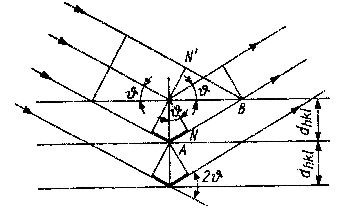
\includegraphics[width=0.3\textwidth]{Abbildungen/Roentgenbeugung.pdf}
    \caption{Beugung eines Röntgenstrahlbündels an einer Netzebenenschar mit Abstand $d_{hkl}$.~\cite[S.367]{Kleber}}
    \label{fig:Roentgenbeugung}
\end{figure}\\
Der Abstand $d$ einer Netzebenschar parallel zum Normalenvektor $\bm{n}=(h,k,l)$ ist abhängig von den Laue-Indizes und den Dimensionen der Elementarzelle und nimmt folgende Form an:
\begin{align}
  d_{hkl} = \frac{1}{\sqrt{\left(\frac{h}{a_0}\right)^2+\left(\frac{k}{b_0}\right)^2+\left(\frac{l}{c_0}\right)^2}}\label{eqn:Ebenabstand}
\end{align}
Für die im Versuch betrachteten kubischen Kristallgitter vereinfacht sich \eqref{eqn:Ebenabstand} zu
\begin{align}
  d_{hkl} = \frac{a_0}{\sqrt{h^2+k^2+l^2}}\label{eqn:Abstand_kubisch}
\end{align}

\subsection{Das Debye-Scherrer Verfahren}
Beim Debye-Scherrer-Verfahren handelt es sich um ein Verfahren der Röntgenfeinstrukturanalyse. Hierbei wird monochromatische Röntgenstrahlung an einem pulverförmigen Präparat gebeugt. Aus den auf einem zylindrisch um die Probe, mit der Zylinderachse senkrecht zur Primärstrahlrichtung, eingelegten Röntgenfilm entstehenden Beugungsringen, deren Entstehung im Folgenden beschrieben wird, lassen sich die \textsc{Bragg}winkel $\vartheta$, der Gitterparameter $a_0$ (für kubische Bravaisgitter) sowie die Millerschen Indizes der jeweiligen Ebenen bestimmen. Damit kann abschließend die Substanz indentifiziert werden.\\
Das \textit{Prinzip} des Versuchs soll mit Hilfe von Abb. \ref{fig:Debye-Kamera} beschrieben werden. Das durch die Blende begrenzte monochromatische Strahlenbündel trifft auf die vorher in Stäbchenform gebrachte Pulverprobe. In dem feinkörnigen Pulver befinden sich unterschiedlich orientierte Kriställchen. Hier finden sich so nun stets Kriställchen, die zufällig so orientiert sind, dass sie für irgendwelche Netzebenenscharen die \textsc{Bragg}'sche Beugungsbedingung~\eqref{eqn:Bragg} für ein festes $\lambda$ und jeweils festes $d$, erfüllen. Durch zusätzliches Drehen der Probe können weitere Variationen der Kistallorientierung erreicht werden.\\
Werden nun alle Kriställchen betrachtet, die für eine bestimmte Netzebenenschar (hkl) zufällig in Reflexionsstellung sind bzw. anders formuliert, die Netzebenen, die wegen der zufällligen Lage des betreffenden Kriställchens mit dem Primärstrahl den nach der \textsc{Bragg}-Bedinung erforderlichen Winkel einschließen, reflektieren diese alle unter dem gleichen Winkel $\vartheta_\text{hkl}$, bzw gleichem Ablenkwinkel $2\cdot\vartheta_\text{hkl}$. Durch die Vielzahl von Kriställchen bzw. Ebenen, an denen die Bedingung erfüllt ist, resultiert aus den sich ergebenden Strahlen ein Kegel um den Primärstrahl mit dem Öffnungswinkel $4\cdot\vartheta_\text{hkl}$. \\
Da d für jede Netzebenenart unterschiedlich ist, treten mehrere Ringe auf dem Röntgenfilm auf. Jeder Debye-Ring entspricht dabei der Reflexion der Wellenlänge an einer Netzebenenart.
\begin{figure}[htp]
    \centering
    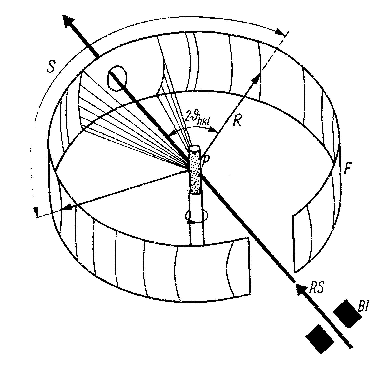
\includegraphics[width=0.3\textwidth]{Abbildungen/Debye-Sherrer-Kamera.pdf}
    \caption{Strahlenverlauf beim Debye-Scherrer-Verfahren.~\cite[S.375]{Kleber}}
    \label{fig:Debye-Kamera}
\end{figure}\\
Um die Schwierigkeit zu umgehen, dass der Filmdurchmesser nicht exakt gleich dem Kameradurchmesser ist (Einfluss der Luftfeuchtigkeit etc.), wird das Verfahren von Straumanis bei der Einlegung des Films verwendet: Dabei wird der Film so in die Kamera eingelegt, dass die Enden des Films in der Zylinderkammer mit dem Primärstrahl einen Winkel von etwa \SI{90}{\degree} einschließen.\\
Bei der \textit{Auswertung} wird nun der Abstand des Ein- und des Austrittsloch (A) bestimmt, der \SI{180}{\degree} entspricht. Mit Hilfe der Verhältnisgleichung
\begin{align}
  \frac{\SI{180}{\degree}}{A} = \frac{4\cdot \vartheta}{ s}\label{eqn:Verhältnisgleichung}
\end{align}
kann dann mit der Kenntnis des Abstandes jeweils zwei zum gleichen Kegel gehörenden Schnittringe $\Delta s$, der \textsc{Bragg}winkel $\vartheta$ bestimmt werden. \\
Für kubische Gitter wird wie folgt vorgegangen: Aus \eqref{eqn:Bragg} und \eqref{eqn:Abstand_kubisch} erhält man durch Quadrierung:
\begin{align}\label{equ:Auswertung}
  \sin^2(\vartheta) = \left(\frac{\lambda}{2\cdot a_0}\right)^2 (h^2+k^2+l^2)
\end{align}
Dabei kann $\sin^2\vartheta$ bei Kenntnis von $\vartheta$ errechnet werden. Beim ersten Faktor auf der rechten Seite handelt es sich um eine Konstante, während der zweite Faktor eine ganze Zahl sein muss. $\sin^2\vartheta$) wird nun als Produkt aus Konstanter und ganzer Zahl dargestellt, wobei bei der ganzen Zahl nur solche möglich sind, die nach den Auslöschungsregeln für das jeweilige Gitter auftreten können. Durch die größtmögliche Anzahl von Relfexen, die auf diese Art zugeordnet werden können, wird die Gitterart und aus der sich ergebenden Konstanten, der Gitterparameter $a_0$ bestimmt.

% ***** Zwei Bilder nebeneinander *****

% \begin{figure}[htp]
%     \centering
%     \begin{subfigure}{0.45\textwidth}
%         \includegraphics[width=\textwidth]{Bilder/Beispielbild.png}
%     \end{subfigure}
%     \begin{subfigure}{0.45\textwidth}
%         \includegraphics[width=\textwidth]{Bilder/Beispielbild.png}
%     \end{subfigure}
%     \caption{Beschreibung}
% \end{figure}

%***** Tabellen *****
% \begin{table}[ht]
% 	\centering
% 	\caption{Überschrift der Tabelle}
% 	\label{tab:Tabelle1}
% 	\begin{tabular}{l c c c}
% 		\toprule
% 	    text & text & text & text\\
% 	 	\midrule
% 			text & text & text & text\\
% 			text & text & text & text
% 	\end{tabular}
% \end{table}

% *********************************************
% ***** KAPITEL 3 *****************************
% *********************************************
\section{Versuchsdurchführung} \label{sec:Versuchsdurchführung}
Für die Aufnahme der zwei Diffraktogramme wurde die kristalline Substanz zunächst mithilfe eines Mörser zu einem kleinen Pulver zerkleinert. Anschließend wurde eine kleine Menge des Pulvers in eine \SI{0.1}{\milli\metre} große Glaskapillare eingefüllt und diese mit einem Klebwachs an der Drehachse der \textsc{Debye\--Sherrer}\--Kamera befestigt. Dabei wurde darauf geachtet, dass die Glaskapillare möglichst senkrecht aufgebracht ist und die Drechachse mittig ausgerichtet ist. Die Justage erfolgte mithilfe eine Justierlupe durchgeführt.
\subsection{Aufnahme der Beugungsbilder}
In der Dunkelkammer wurde unter Rotlicht der Röntgenfilm in die Kamera eingelegt, sowie Primärstrahlfänger und Blende wieder eingesetzt. Beim Einlegen des Films wurde mit einer Schere die untere rechte Ecke des Films abgeschnitten, um die Orientierung des Films innerhalb der Kamera später rekonstruieren zu können.\\
Im weiteren Verlauf wurde die \textsc{Debye\--Sherrer}\--Kamera auf die entsprechende Halterung in der Röntgenkamera gesetzt und der Motor zur Drehung des Präparats montiert.\\
Für die Aufnahmen wurde eine Hochspannung von \SI{35}{\kilo\volt} mit einem Anodenstrom von \SI{30}{\milli\ampere} eingestellt. Die erste Probe wurde ohne Filter 10 Minuten lang beleuchtet.\\
Für die zweite Probe wurde ein Nickel-Filter eingesetzt und insgesamt 30 Minuten lang beleuchtet.
\subsection{Entwicklung des Röntgenfilms}
Nach der Beleuchtung der Probe wurde der Röntgenfilm in der Dunkelkammer aus der Kamera herausgeholt und entwickelt. Dafür wurde der Film für 4 Minuten in das Entwicklerbad getaucht. Dabei wurde der Film immer wieder leicht bewegt, um eine gleichmäßige Wirkung der Entwicklersubstanz zu gewährleisten.\\
Anschließend wurde der Film kurz in einem Wasserbad gewässert und anschließend für 15 Minuten in ein Fixierbad getaucht. Zuletzt wurde der Film erneut für weitere 20 Minuten in das Wasserbad gebracht und im Anschluss noch mit Netzmittel behandelt.


% *********************************************
% ***** KAPITEL 4 *****************************
% *********************************************
\newpage
\section{Ergebnisse und Diskussion}
Es wurden zwei Difraktogramme einer gegebenen unbekannten polykristallinen kubischen Substanz mit einer Debye-Scherrer Kamera aufgenommen. Dabei wurde die Messung einmal mit und einmal ohne einen Nickel-Absorptionsfilter zur Herausfilterung der $K_{\beta}$ Linie durchgeführt. Im Vergleich beider Difraktogramme wird nach Ausmessen der Linien festgestellt, dass sowohl mit- als auch ohne Filter die gleiche Anzahl von Linien auftreten. Daraus kann geschlussfolgert werden, dass es sich bei allen auch ohne Filter auftretenden Linien um $K_{\alpha}$-Linien handelt.
\subsection{Salzstruktur mit Nickelfilter}
\subsubsection{Indizierung der Reflexe}
Zuerst wird ein kristallines Salz untersucht, indem die Beugungsringe auf dem Röntgenfilm ausgemessen werden. Zunächst wird der Röntgenfilm dafür eingescannt. Das zugehörige Bild zeigt Abbildung~\ref{fig:Film_mitFilter}.
\begin{figure}[htp]
    \centering
        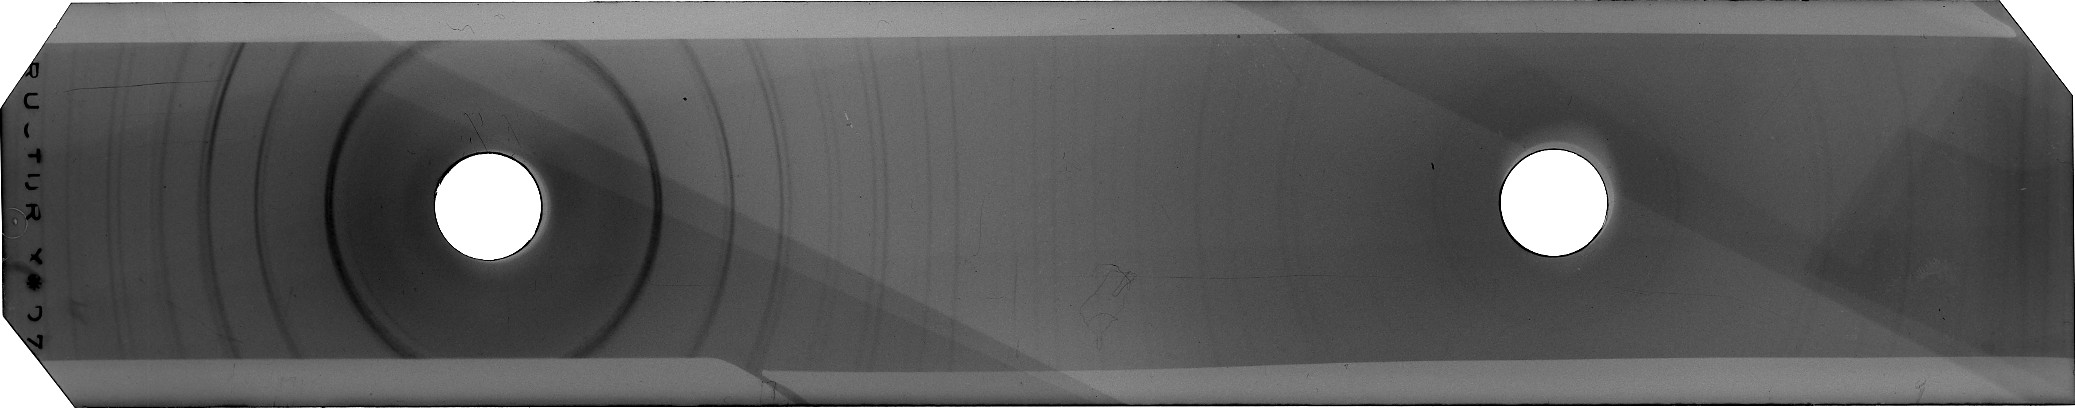
\includegraphics[width=0.9\textwidth]{Abbildungen/Roentgenfilm_mit_Filter.jpg}
    \caption{Eingescannter Röntgenfilm der Aufnahme mit Verwendung eines Nickelfilters und einer Belichtungszeit von \SI{30}{\minute}.}
    \label{fig:Film_mitFilter}
\end{figure}\\
Die deutlich erkennbaren Streifen entstanden wahrscheinlich durch Belichtung der Filme mit normalen Licht, als sich ein weiterer Filmstreifen schräg über dem Röntgenfilm befand. Dieser Streifen hat jedoch keinen Einfluss auf das Ausmessen der Beugungsringe.\\
Jeweils rechts und links des Fängerloches wird die Position der Beugungsringe mithilfe des Programms \textit{ImageJ} entlang einer festen manuell eingefügten Mittellinie bestimmt und durch Mittelwertbildung die Position des Fängerloches berechnet. Die gleiche Berechnung erfolgte für die Beugungsringe um das Strahleingangsloch. Der Abstand beider Löcher ergab sich zu:
\begin{align}
  A = \SI{3,529\pm 0,013}{\text{inch}}.
\end{align}
Aufgrund der großen Anzahl an Beugungsringen erfolgte die Bestimmung des Fehlers für die Positionen der Strahllöcher durch statistische Auswertung der bestimmten Positionen und anschließende Addition der Fehler. Der Abstand $A$ entspricht \SI{180}{\degree} in der Kamera, da sich beide Punkte genau gegenüberliegen. Aus der Verhältnisgleichung~\eqref{eqn:Verhältnisgleichung} lässt sich nun der \textsc{Bragg}-Winkel jedes Beugungsringes aus dem Durchmesser $s$ berechnen
\begin{align}
  \vartheta &= \frac{\SI{180}{\degree}s}{4\cdot A}\\
  \Delta \vartheta &= \frac{\SI{180}{\degree}}{4}\left[\frac{\Delta s}{A} + \frac{s\Delta A}{A^2}\right].
\end{align}
Zur Bestimmung der Gitterkonstanten wird wie in \ref{sec:Verfahren} beschrieben, vorgegangen. Der konstante Faktor auf der linken Seite von Gleichung \ref{equ:Auswertung}
wird als:
\begin{align}
  Q :=\frac{\lambda^2}{4 a_0^2} = \frac{\sin^2(\vartheta)}{h^2 + k^2+l^2}\label{eqn:Q_Parameter}
\end{align} definiert. Die Messergebnisse dazu zeigt Tabelle~\ref{tab:Q_Paramter}.
\begin{table}[ht]
	\centering
	\caption{Durchmesser $s$ der Beugungsringe und daraus berechnete Beugungswinkel $\vartheta$. Mithilfe der Beugungswinkel lässt sich durch Indizierung die Konstante $Q$ durch Ausklammern der ganzen Zahl $n = h^2 +k^2 +l^2$ ermitteln.}
	\label{tab:Q_Paramter}
	\begin{tabular}{l c c c c c | c c c c}
		\toprule
      Nr. & $s [\text{inch}]$ & Intensität & $\vartheta [\si{\degree}]$ & $\Delta \vartheta [\si{\degree}]$ & $\sin^2 \vartheta $ & $Q$ & $(hkl)$ & $n$ & $a_0 [\si{\textup{\AA}}]$\\
    \midrule
1  & 0,99 & hell      & 12,60 & 0,30 & 0,0476 &         &     &    &       \\
2  & 1,09 & dunkel    & 13,90 & 0,56 & 0,0577 & 0,02884 & 110 & 2  & 4,538 \\
3  & 1,55 & hell      & 19,76 & 0,33 & 0,1143 & 0,02858 & 200 & 4  & 4,559 \\
4  & 1,59 & dunkel    & 20,27 & 0,33 & 0,1201 &         &     &    &       \\
5  & 1,91 & dunkel    & 24,35 & 0,34 & 0,1700 & 0,02834 & 211 & 6  & 4,579 \\
6  & 1,96 & hell      & 24,99 & 0,35 & 0,1785 &         &     &    &       \\
7  & 2,23 & hell      & 28,43 & 0,36 & 0,2267 & 0,02834 & 220 & 8  & 4,579 \\
8  & 2,30 & hell      & 29,33 & 0,36 & 0,2399 &         &     &    &       \\
9  & 2,52 & hell      & 32,13 & 0,37 & 0,2829 & 0,02829 & 310 & 10 & 4,583 \\
10 & 2,59 & hell      & 33,02 & 0,37 & 0,2970 &         &     &    &       \\
11 & 2,80 & sehr hell & 35,70 & 0,38 & 0,3405 & 0,02838 & 222 & 12 & 4,576 \\
12 & 2,87 & hell      & 36,59 & 0,39 & 0,3554 &         &     &    &       \\
13 & 3,05 & hell      & 38,89 & 0,40 & 0,3941 &         &     &    &       \\
14 & 3,21 & hell      & 40,91 & 0,40 & 0,4288 &         &     &    &       \\
15 & 3,59 & hell      & 45,79 & 0,77 & 0,5139 & 0,02855 & 330 & 18 & 4,562 \\
16 & 3,71 & hell      & 47,32 & 0,77 & 0,5405 & 0,02845 & 331 & 19 & 4,570 \\
17 & 3,85 & hell      & 49,11 & 0,78 & 0,5715 & 0,02857 & 420 & 20 & 4,560 \\
18 & 3,99 & hell      & 50,89 & 0,79 & 0,6021 & 0,02867 & 421 & 21 & 4,552 \\
19 & 4,11 & hell      & 52,42 & 0,79 & 0,6281 & 0,02855 & 332 & 22 & 4,562 \\
20 & 4,29 & hell      & 54,68 & 0,78 & 0,6658 &         &     &    &       \\
21 & 4,41 & hell      & 56,18 & 0,81 & 0,6901 & 0,02876 & 422 & 24 & 4,545 \\
22 & 4,68 & hell      & 59,65 & 0,80 & 0,7448 & 0,02864 & 431 & 26 & 4,554 \\
23 & 4,87 & hell      & 62,08 & 0,94 & 0,7807 &         &     &    &       \\
24 & 5,22 & hell      & 66,54 & 0,95 & 0,8415 &         &     &    &       \\
25 & 5,31 & hell      & 67,69 & 0,96 & 0,8559 & 0,02853 & 521 & 30 & 4,563 \\
26 & 6,25 & dunkel    & 79,67 & 0,87 & 0,9679 & 0,02847 & 433 & 34 & 4,564 \\
27 & 6,31 & hell      & 80,44 & 0,87 & 0,9724 & 0,02860 & 530 & 34 & 4,566
	\end{tabular}
\end{table}\\
Zur Bestimmung der Konstanten $Q$ muss eine Indizierung der Reflexe durchgeführt werden. Dafür wird jeder Term von $\sin^2 \vartheta $ durch eine ganze Zahl $n = h^2 + k^2 + l^2$ geteilt, sodass das entsprechende Ergebnis für alle Messwerte eine Konstante ist. Dies wird für alle gemessenen Reflexe durchgeführt und dabei festgestellt, dass einige Winkel nah beeinander liegen und die Indizierung der beiden Reflexe mit einer einzigen Konstanten $Q$ nicht möglich ist. Die Reflexe unterscheiden sich auch nicht speziell durch ihre Intensität von den restlichen Ergebnissen, weshalb Reflexe, die durch die $K_\beta$-Linie des Röntgenspektrums verursacht werden, dafür ausgeschlossen werden können. Es wird davon ausgegangen, dass bei den Werten, wo keine Indizierung möglich war, Messfehler auftraten. Beispielsweise können Reflexe durch die Beugung der Röntgenstrahlen am Messing der Blendenvorrichtung entstehen.
\subsubsection{Auslöschungsregeln}\label{sec:Auslöschungsregeln}
Für die Bestimmung der Gitterstruktur wird untersucht, welche Reflexe für bestimmte Kristallgitterarten auftreten können. Dies wird durch die \textit{Auslöschungsregeln} beschrieben. Für Raumzentrierte Gitter muss die Summe der Indizes $(hkl)$ eine gerade Zahl sein. Bei Raumzentrierten Gittern muss jeweils die Summe zweier Indizes gerade sein. Da für kubisch primitive Gitter nur ein Atom pro Elementarzelle vorhanden ist, sind alle möglichen Kombinationen von $(hkl)$ möglich. Dies lässt sich zusammenfassen zu:
\begin{align}
  \text{Innenzentriert:} & \qquad h + k +l = 2n\nonumber\\
  \text{Raumzentriert:}  & \qquad h, k, l \text{ alle gerade oder ungerade}\\
  \text{Primitiv:} & \qquad h, k, l \text{ beliebig}\nonumber
\end{align}
Werden nun also die möglichen Kombinationen von $(hkl)$ den einzelnen Gitterstrukturen zugeordnet, ergibt sich die in Tabelle \ref{tab:Indizierung} gezeigte Übersicht.
\begin{table}[ht]
	\centering
	\caption{Darstellung der möglichen $(hkl)$ Kombinationen für verschiedene Gitterarten. Es gilt $n = h^2+k^2+l^2$.}
	\label{tab:Indizierung}
	\begin{tabular}{c c c l c c c l c c c l}
		\toprule
      \multicolumn{4}{c}{Primitiv} & \multicolumn{4}{c}{Flächenzentriert} & \multicolumn{4}{c}{Raumzentriert}\\
      \cmidrule(lr){1-4}\cmidrule(lr){5-8}\cmidrule(lr){9-12}
      h & k & l & n & h & k & l & n & h & k & l & n \\
      \midrule
      1 & 0 & 0 & 1   & 1 & 1 & 1 & 3   & 1 & 1 & 0 & 2   \\
      1 & 1 & 0 & 2   & 2 & 0 & 0 & 4   & 2 & 0 & 0 & 4   \\
      1 & 1 & 1 & 3   & 2 & 2 & 0 & 8   & 2 & 1 & 1 & 6   \\
      2 & 0 & 0 & 4   & 3 & 1 & 1 & 11  & 2 & 2 & 0 & 8   \\
      2 & 1 & 0 & 5   & 2 & 2 & 2 & 12  & 3 & 1 & 0 & 10  \\
      2 & 1 & 1 & 6   & 4 & 0 & 0 & 16  & 2 & 2 & 2 & 12  \\
      2 & 2 & 1 & 9   & 3 & 3 & 1 & 19  & 3 & 2 & 1 & 14  \\
      2 & 2 & 2 & 12  & 4 & 2 & 0 & 20  & 4 & 0 & 0 & 16  \\
      3 & 2 & 1 & 14  & 4 & 2 & 2 & 24  & 3 & 3 & 0 & 18  \\
      3 & 2 & 2 & 17  & 3 & 3 & 3 & 27  & 4 & 1 & 1 & 18  \\
      3 & 3 & 2 & 22  & 5 & 1 & 1 & 27  & 4 & 2 & 0 & 20  \\
      3 & 3 & 3 & 27  & 4 & 4 & 0 & 32  & 3 & 3 & 2 & 22  \\
      4 & 1 & 1 & 18  & 5 & 3 & 3 & 43  & 5 & 2 & 1 & 30  \\
      4 & 2 & 1 & 21  & 4 & 4 & 4 & 48  & 4 & 4 & 0 & 32
	\end{tabular}
\end{table}\\
In Tabelle \ref{tab:Q_Paramter} werden bereits alle möglichen Indizierungen gezeigt, für welche ein mögliches $n = h^2+ k^2 +l^2$ auftreten können. Es stellt sich heraus, dass besonders viele Werte von $n$ in \ref{tab:Q_Paramter} geradzahlig sind, was auf kubisch innenzentrierten Gittercharakter hindeutet. Da jedoch auch ungerade $n$ auftauchen, wird auf ein kubisch primitves Gitter geschlossen.\\
\subsubsection{Bestimmung der Gitterkonstante}
Die Gitterkonstante des primitiven Gitters ergibt sich nun aus der Konstanten $Q$ und der Wellenlänge $\lambda$.\\
Für die Wellenlänge wurde bei den ersten 25 Werten eine gemittelte Wellenlänge der $K_\alpha$- und $K_\beta$-Linie angenommen. Diese berechnet sich durch
\begin{align}
  \lambda_{K_\alpha} = \frac{2\lambda_{K_{\alpha_1}}+\lambda_{K_{\alpha_2}}}{3}
\end{align}
Für die $K_\alpha$-Linien von Kupfer gelten folgende Literaturwerte
\begin{align}
  \lambda_{K_{\alpha_1}} &= \SI{1,54015}{\textup{\AA}}\nonumber\\
  \lambda_{K_{\alpha_2}} &= \SI{1,54433}{\textup{\AA}}\label{eqn:Wellenlänge}\\
\Rightarrow \lambda_{K_\alpha} &= \SI{1,54154}{\textup{\AA}}.\nonumber
\end{align}
Die Formel der Gitterkonstante ergibt sich mithilfe von \eqref{eqn:Q_Parameter}
\begin{align}
  a_0 &= \frac{\lambda}{2 \sqrt{Q}}\\
  \Delta a_0 &= \frac{1}{2\sqrt{Q}} \left[\Delta \lambda + \frac{\lambda \Delta Q}{\sqrt{Q}}\right].
\end{align}
Nach \eqref{eqn:Q_Parameter} folgt für den Fehler des Q-Parameters und für die Gitterkonstante
\begin{align}
  \Delta Q &= \frac{2 \sin(\vartheta)\Delta \vartheta}{h^2+k^2+l^2}\\
  \Rightarrow \Delta a_0 &= \frac{1}{2\sqrt{Q}} \left[\Delta \lambda + \frac{\lambda 2 \sin(\vartheta)\Delta \vartheta}{n\sqrt{Q}}\right] \quad \text{mit }n = h^2+k^2+l^2.
\end{align}
Für Reflexe mit großem Beugungswinkel ist die Dispersion am größten und bereits kleine Änderungen der Wellenlänge bewirken eine sichtbaren Unterschied des Beugungswinkels
\begin{align}
  \Delta \lambda = 2 \Delta d \sin(\vartheta) \qquad (\text{für konstantes }\vartheta).
\end{align}
Somit lässt sich für die Reflexe mit dem größten Beugungswinkel die Feinstrukturaufspaltung von $K_{\alpha_1}$ und $K_{\alpha_2}$ beoachten. Die Reflexe 26 und 27 haben die größten gemessenen \textsc{Bragg}-Winkel und liegen nah beeinander, weshalb für Reflex 26 die Wellenlänge der $K_{\alpha_1}$-Linie und für Reflex 27 die Wellenlänge der $K_{\alpha_2}$-Linie zur Berechnung der Gitterkonstante genutzt wird.
Die Ergebnisse der Rechnungen werden in Tabelle~\ref{tab:Ergebnisse} nochmal ausführlich dargestellt. Es wurde auf die nicht-indizierbaren Reflexe verzichtet.
\begin{table}[ht]
	\centering
	\caption{Beugungswinkel an den Netzebenen mit Parametern $(hkl)$ und daraus berechnete Gitterkonstante $a_0$.}
	\label{tab:Ergebnisse}
	\begin{tabular}{l c c c c}
		\toprule
      Nr. & $\vartheta~[\si{\degree}]$ & $(hkl)$ & $a_0~[\si{\textup{\AA}}]$ & $\Delta a_0~[\si{\textup{\AA}}]$\\
    \midrule
    1  & 13,90 & 110 & 4,538 & 0,113 \\
    2  & 19,76 & 200 & 4,559 & 0,042 \\
    3  & 24,35 & 211 & 4,579 & 0,054 \\
    5  & 28,43 & 220 & 4,579 & 0,051 \\
    7  & 32,13 & 310 & 4,583 & 0,049 \\
    9  & 35,70 & 222 & 4,576 & 0,048 \\
    11 & 45,79 & 330 & 4,562 & 0,073 \\
    16 & 47,32 & 331 & 4,570 & 0,072 \\
    17 & 49,11 & 420 & 4,560 & 0,071 \\
    18 & 50,89 & 421 & 4,552 & 0,070 \\
    19 & 52,42 & 332 & 4,562 & 0,069 \\
    21 & 56,18 & 422 & 4,545 & 0,068 \\
    22 & 59,65 & 431 & 4,554 & 0,059 \\
    25 & 67,69 & 521 & 4,563 & 0,064 \\
    26 & 79,67 & 433 & 4,564 & 0,059 \\
    27 & 80,44 & 530 & 4,566 & 0,059
	\end{tabular}
\end{table}
\subsubsection{Korrektur nach Hadding}
Findet eine hohe Absorption der Probe statt, dann tritt die \textsc{Bragg}-Reflexion fast nur an der Oberfläche der Probe auf, sodass sich die Radien der beobachtbaren Ringe auf dem Röntgenfilm verändern. Nach \textsc{Hadding} lässt sich, da von einer völlig undurchlässigen Probe ausgegangen wird, dieser Fehler folgendermaßen korrigieren:
\begin{align}
  2r_\text{korr} = 2r - \rho (1+\cos(2\vartheta))
\end{align}
Dabei ist $r_\text{korr}$ der korrigierte Ringradius, $r$ der gemessene Radius der Beugungsringe, $\vartheta$ der gemessene \textsc{Bragg}-Winkel und $\rho$ beschreibt den Radius der Probe. Im Experiment wurde der Durchmesser der Glaskapillare auf
\begin{align}
  2\rho = \SI{0,1}{\milli\metre} = \SI{3,937e-3}{\text{inch}}
\end{align}
bestimmt. Mit dieser Korrektur wurden die \textsc{Bragg}-Winkel neu berechnet und daraus eine korrigierte Gitterkonstante bestimmt. Die Ergebnisse sind in Tabelle~\ref{tab:Hadding} dargestellt.
\begin{table}[ht]
	\centering
	\caption{Korrektur des Durchmessers $s_\text{korr}$ der Beugungsringe und daraus berechnete Gitterkonstanten.}
	\label{tab:Hadding}
	\begin{tabular}{l c c c c c}
		\toprule
      Nr. & $s_\text{korr}$ & $\vartheta_\text{korr}~[\si{\degree}]$ & $Q_\text{korr}$ & $a_{0,\text{korr}}~[\si{\textup{\AA}}]$ & $\Delta a_{0,\text{korr}}~[\si{\textup{\AA}}]$\\
    \midrule
    2  & 1,09 & 13,9 & 0,0287 & 4,553 & 0,114 \\
    3  & 1,55 & 19,7 & 0,0285 & 4,569 & 0,059 \\
    5  & 1,91 & 24,3 & 0,0282 & 4,586 & 0,054 \\
    7  & 2,23 & 28,4 & 0,0283 & 4,585 & 0,051 \\
    9  & 2,52 & 32,1 & 0,0282 & 4,588 & 0,049 \\
    11 & 2,80 & 35,7 & 0,0283 & 4,579 & 0,048 \\
    14 & 3,21 & 40,9 & 0,0286 & 4,561 & 0,046 \\
    16 & 3,71 & 47,3 & 0,0284 & 4,572 & 0,072 \\
    17 & 3,85 & 49,1 & 0,0286 & 4,561 & 0,071 \\
    18 & 3,99 & 50,9 & 0,0287 & 4,553 & 0,070 \\
    19 & 4,11 & 52,4 & 0,0285 & 4,563 & 0,069 \\
    21 & 4,40 & 56,2 & 0,0287 & 4,546 & 0,068 \\
    22 & 4,68 & 59,6 & 0,0286 & 4,555 & 0,059 \\
    25 & 5,31 & 67,7 & 0,0285 & 4,564 & 0,064 \\
    26 & 6,25 & 79,7 & 0,0285 & 4,564 & 0,059 \\
    27 & 6,31 & 80,4 & 0,0286 & 4,566 & 0,059
	\end{tabular}
\end{table}

\subsubsection{Extrapolation, Gitterkonstanten- und Substanzbestimmung}
Bei der Messung können mehrere systematische Fehler auftreten, deren Einfluss durch geeignete Extrapolation eliminiert wird.\\ Als ein systematischer Fehler ist aufzuführen, dass die Lage der Debye-Ringe stark von der Absorption des Präparats abhängig ist. Hierbei wird die Verschiebung der Debye-Ringe mit zunehmendem Bragg-Winkel kleiner und bei $\vartheta$ = \SI{90}{\degree} ist keine Verschiebung mehr festzustellen. \\
Einen weiteren systematischen Fehler, der die Lage der Beugungsringe beeinflusst, stellt die Kameraverzerrung dar. Auch diese ist winkelabhängig und minimal für $\vartheta$ = \SI{90}{\degree}\\
Um diese bei der Gitterkonstantenbestimmung zu eliminieren, wird eine im Bereich von $\SI{60}{\degree} \leq \vartheta \geq \SI{90}{\degree}$ annährend linear verlaufende und bei $\vartheta$ = \SI{90}{\degree} den Wert Null annehmende Extrapolationsfunktion - die Nelson-Riley-funktion- verwendet: \\
\begin{align}
  a_{0,hkl,gemessen} = f(\frac{1}{2}\cdot[\frac{cos^2(\vartheta)}{\vartheta}+\frac{cos^2(\vartheta)}{sin(\vartheta)}])
\end{align}

Werden nun die $a_{0}$-Werte, die zu $\vartheta$ gehören, für das gilt $\SI{60}{\degree} \leq \vartheta \geq \SI{90}{\degree}$ über der sich aus $(\frac{1}{2}\cdot[\frac{cos^2(\vartheta)}{\vartheta}+\frac{cos^2(\vartheta)}{sin(\vartheta)}])$ ergebenden Abzissenachsenwerten aufgetragen und mit einer linearen Funktion gefittet, lässt sich der korrigierte Wert der Gitterkonstanten aufgrund obiger Überlegungen als Schnittpunkt mit der Ordinatenachse ablesen. In der durchgeführten Extrapolation \ref{fig:Extrapolation} wurden dabei Winkel für $\vartheta$ $\SI{56,18}{\degree} \leq \vartheta \geq \SI{80,44}{\degree}$ verwendet.

\begin{figure}[htp]
    \centering
    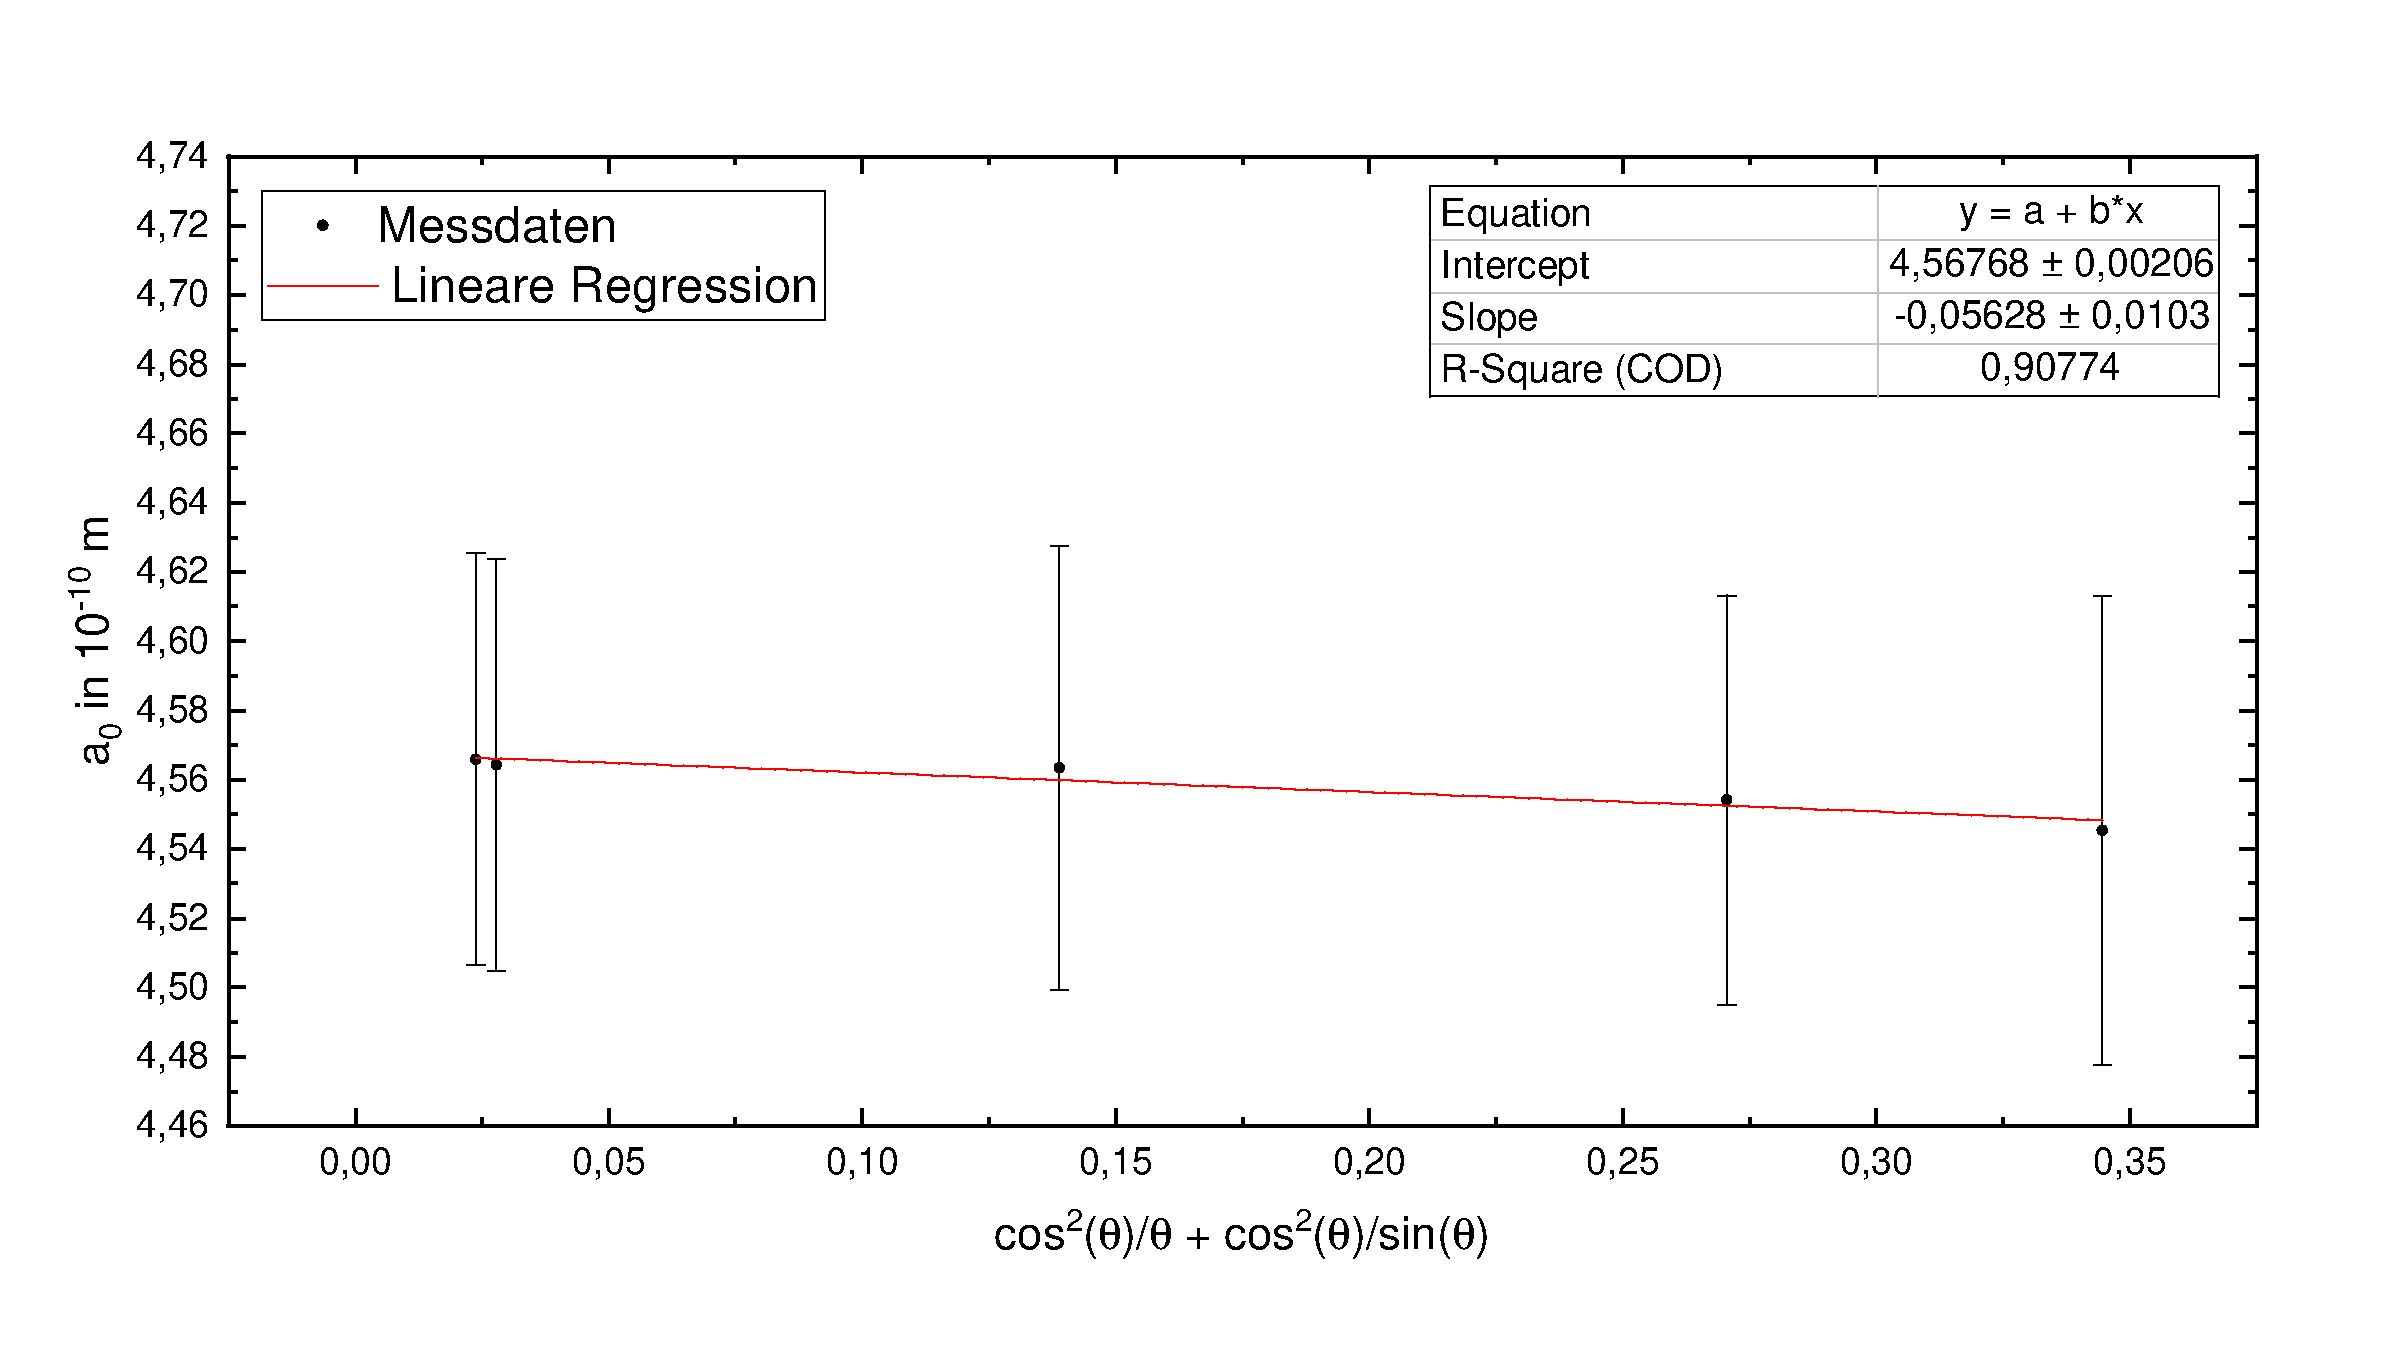
\includegraphics[width=0.9\textwidth]{Abbildungen/Extrapolation_anichtkorr.pdf}
    \caption{Gitterparameter $a_{0}$ über Nelson-Riley-Funktion zur Extrapolation.}
    \label{fig:Extrapolation}
\end{figure}\\
\FloatBarrier
Aus der Extrapolation ergibt sich für
\begin{align}\label{equ:a01}
   a_{0} = \SI{4,568 \pm 0,002}{\textup{\AA}}
\end{align}

Als Vergleich wird der beim größten $\vartheta$-Wert errechnete Gitterparamter $a_{0}$ herangezogen, da hier der systematische Fehler aufgrund obiger Diskussion am kleinsten ist:
\begin{align}\label{equ:a02}
   a_{0} = \SI{4,566 \pm 0,059}{\textup{\AA}}
\end{align}

Dieser entspricht auch dem nach der Hadding-Korrektur errechneten Wert für $a_0$. Diese ist also als zur Bestimmung der Gitterkonstanten als wenig sinnvoll einzuschätzen, da sie für große Winkel, die für eine Bestimmung der Gitterkonstanten betrachtet werden, keine Korrektur mehr bewirkt. \\

Aufgrund des so ermittelten Gitterparameters lässt sich die untersuchte unbekannte Substanz als Cäsium-Iodid bestimmen. Dieses hat eine Gitterkonstante von
\begin{align}
  a_{0} = \SI{0,4567}{\nano\meter} = \SI{4,567}{\textup\AA}      \cite{Uschmann}
\end{align}

welches sowohl im Fehlerintervall von \ref{equ:a01}, als auch in dem von \ref{equ:a02} liegt. \\
Cäsium-Iodid hat ein kubisch primitives Bravaisgitter. Auch dies zeigt sich in den Messergebnissen. In \ref{sec:Auslöschungsregeln} wird auf ein kubisch primitves Gitter geschlossen, welches jedoch kubisch innenzentrierte Tendenzen aufweist. Letzteres wird bei einer Betrachtung des Atomformfaktors beider Elemente erklärbar: Cäsium (Atomformfaktor bei $\frac{\sin(\theta)}{\lambda} = \SI{0.6}{\textup{\AA}}: 26,5 \; \cite{Uschmann}$, Anhang D ) und Iod (Atomformfaktor bei $\frac{\sin(\theta)}{\lambda} = \SI{0.6}{\textup{\AA}}: 25,3 \; \cite{Uschmann}$, Anhang D) haben sehr ähnliche Atomformfaktoren, weshalb es, obwohl es ein zweiatomiges kubisch primitives Gitter ist, teilweise als kubisch flächenzentriertes Gitter beugt.

\FloatBarrier
\subsection{Salzstruktur ohne Nickelfilter}
Von der gleichen Salzprobe wurde ebenfalls eine Aufnahme ohne Nickelfilter aufgenommen. Die Belichtungszeit war mit $\SI{10}{\min}$ kürzer, weshalb die aufgenommen Ringe weniger gut zu sehen sind (siehe Abb.~\ref{fig:Film_ohneFilter}).
\begin{figure}[htp]
    \centering
        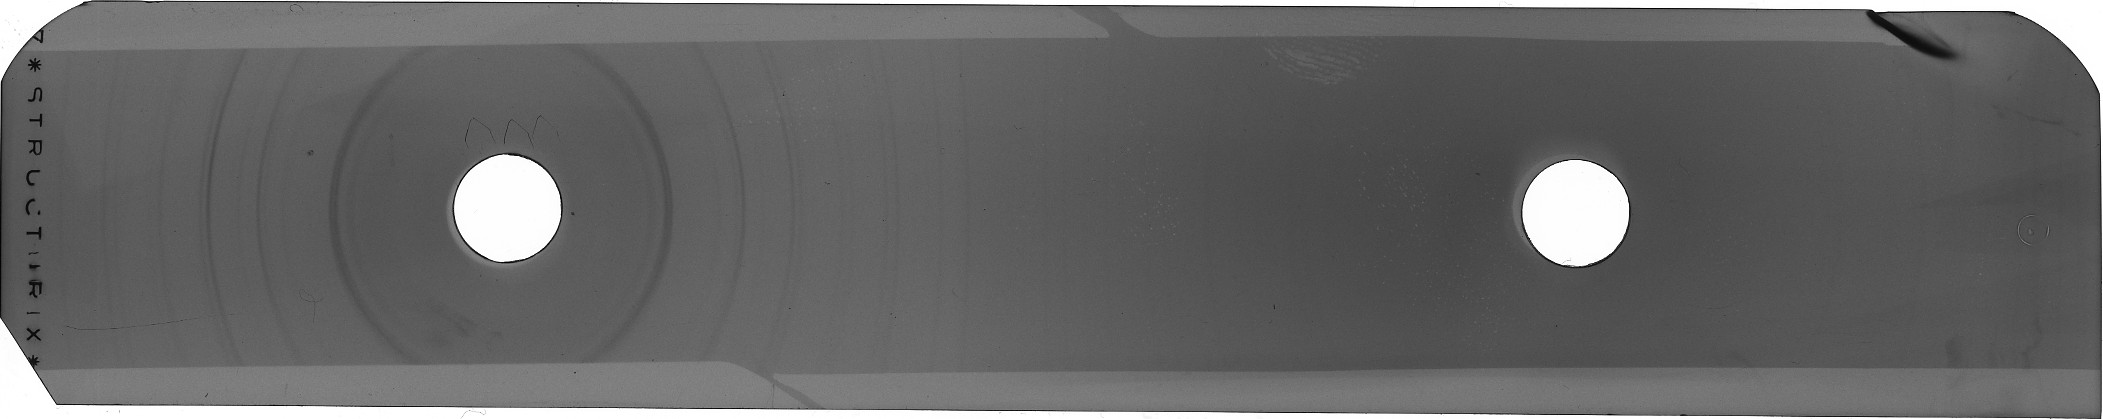
\includegraphics[width=0.9\textwidth]{Abbildungen/Roentgenfilm_ohne_Filter.jpg}
    \caption{Eingescannter Röntgenfilm der Aufnahme mit Verwendung eines Nickelfilters und einer Belichtungszeit von \SI{30}{\minute}.}
    \label{fig:Film_ohneFilter}
\end{figure}\\
Durch Kontrasterhöhung des Scans lassen sich die Reflexe um das Strahleintrittsloch trotzdem auslesen. Die Ergebnisse sind in Tabelle~\ref{tab:Ergebnisse_ohneFilter} dargestellt.
\begin{table}[ht]
	\centering
	\caption{Durchmesser $s$ der Beugungsringe und daraus berechnete Beugungswinkel $\vartheta$. Für die Bestimmung von $s$ wurde die \textsc{Hadding}-Korrektur angewandt. Die Parameter $Q$ wurden indiziert und daraus die Gitterkonstante $a_0$ bestimmt.}
	\label{tab:Ergebnisse_ohneFilter}
	\begin{tabular}{l c c c c c | c c c c c }
		\toprule
      Nr. & $s [\text{inch}]$ & Intensität & $\vartheta [\si{\degree}]$ & $\Delta \vartheta [\si{\degree}]$ & $\sin^2 \vartheta $ & $Q$ & $(hkl)$ & $n$ & $a_0 [\si{\textup{\AA}}]$ & $\Delta a_0 [\si{\textup{\AA}}]$\\
    \midrule
    1  & 0,9963 & hell         & 12,69 & 0,27 & 0,0482 & 0,024 &     &    &       &       \\
    2  & 1,1113 & dunkel       & 14,15 & 0,48 & 0,0598 & 0,030 & 110 & 2  & 0,205 & 0,166 \\
    3  & 1,4565 & hell         & 18,55 & 0,34 & 0,1012 & 0,051 &     &    &       &       \\
    4  & 1,5765 & hell         & 20,07 & 0,36 & 0,1178 & 0,029 & 200 & 4  & 0,172 & 0,094 \\
    5  & 1,6166 & dunkel       & 20,58 & 0,37 & 0,1236 & 0,031 &     &    &       &       \\
    6  & 1,7466 & sehr hell    & 22,24 & 0,38 & 0,1433 & 0,029 & 210 & 5  & 0,163 & 0,093 \\
    7  & 1,9468 & dunkel       & 24,79 & 0,41 & 0,1758 & 0,029 & 211 & 6  & 0,155 & 0,090 \\
    8  & 1,9968 & heller       & 25,43 & 0,42 & 0,1843 & 0,031 &     &    &       &       \\
    9  & 2,2770 & mitteldunkel & 28,99 & 0,46 & 0,2349 & 0,029 & 220 & 8  & 0,143 & 0,087 \\
    10 & 2,3370 & heller       & 29,76 & 0,47 & 0,2463 & 0,031 &     &    &       &       \\
    11 & 2,5672 & heller       & 32,69 & 0,51 & 0,2917 & 0,029 & 310 & 10 & 0,135 & 0,086 \\
    12 & 2,6473 & dunkler      & 33,71 & 0,52 & 0,3080 & 0,028 &     &    &       &       \\
    13 & 2,9375 & dunkler      & 37,40 & 0,56 & 0,3690 & 0,028 & 320 & 13 & 0,126 & 0,086 \\
    14 & 3,1177 & dunkler      & 39,70 & 0,59 & 0,4080 & 0,029 &     &    &       &       \\
    15 & 3,6313 & hell         & 46,24 & 1,59 & 0,5216 & 0,029 &     &    &       &       \\
    16 & 3,6864 & hell         & 46,94 & 0,67 & 0,5338 & 0,028 &     &    &       &       \\
    17 & 3,8365 & hell         & 48,85 & 0,69 & 0,5670 & 0,028 & 420 & 20 & 0,110 & 0,086 \\
    18 & 4,0367 & hell         & 51,40 & 0,72 & 0,6108 & 0,029 &     &    &       &       \\
    19 & 4,1618 & hell         & 52,99 & 1,67 & 0,6377 & 0,029 & 332 & 22 & 0,106 & 0,177 \\
    20 & 4,3219 & hell         & 55,03 & 1,69 & 0,6715 & 0,028 &     &    &       &       \\
    21 & 4,4220 & hell         & 56,31 & 1,71 & 0,6922 & 0,029 &     &    &       &       \\
    22 & 4,6772 & hell         & 59,56 & 0,82 & 0,7432 & 0,029 & 431 & 26 & 0,100 & 0,088 \\
    23 & 4,8874 & hell         & 62,23 & 0,85 & 0,7829 & 0,029 &     &    &       &       \\
    24 & 5,2176 & hell         & 66,44 & 0,90 & 0,8402 & 0,029 &     &    &       &       \\
    25 & 5,3076 & hell         & 67,58 & 0,91 & 0,8546 & 0,028 & 521 & 30 & 0,094 & 0,091 \\
    26 & 6,2681 & hell         & 79,81 & 1,05 & 0,9687 & 0,028 & 530 & 34 & 0,086 & 0,097
	\end{tabular}
\end{table}\\
Wie bereits am Anfang diskutiert, lassen sich bei dem Röntgenfilm ohne Filter ähnlich viele Reflexe feststellen. Im Vergleich fällt auf, dass die gemessenen Beugungswinkel $\vartheta$ im Fehlerintervall mit den Beugungswinkeln der anderen Messung übereinstimmen. Da sich bei der Messung keine Reflexe feststellen lassen, welche auf dem Röntgenfilm ohne Nickelfilter fehlen, kann ausgeschlossen werden, dass Reflexe von der $K_\beta$-Linie der Kupferanode verursacht wurden.\\
Cäsiumiodid wirkt sehr fluoreszierend und führt deshalb zu einer leichten Schwärzung des gesamten Röntgenfilms, was zu einer Überdeckung der schwachen $K_\beta$ Reflexe führen kann.
\FloatBarrier
\subsection{Metalldraht mit Nickelfilter}
Als weitere Probe wurde ein dünner Metalldraht verwendet, und der Röntgenfilm wurde $\SI{25}{\min}$ beleuchtet. Das entstandene Beugungsmuster ist in Abbildung~\ref{fig:Metalldraht} dargestellt.
\begin{figure}[htp]
    \centering
        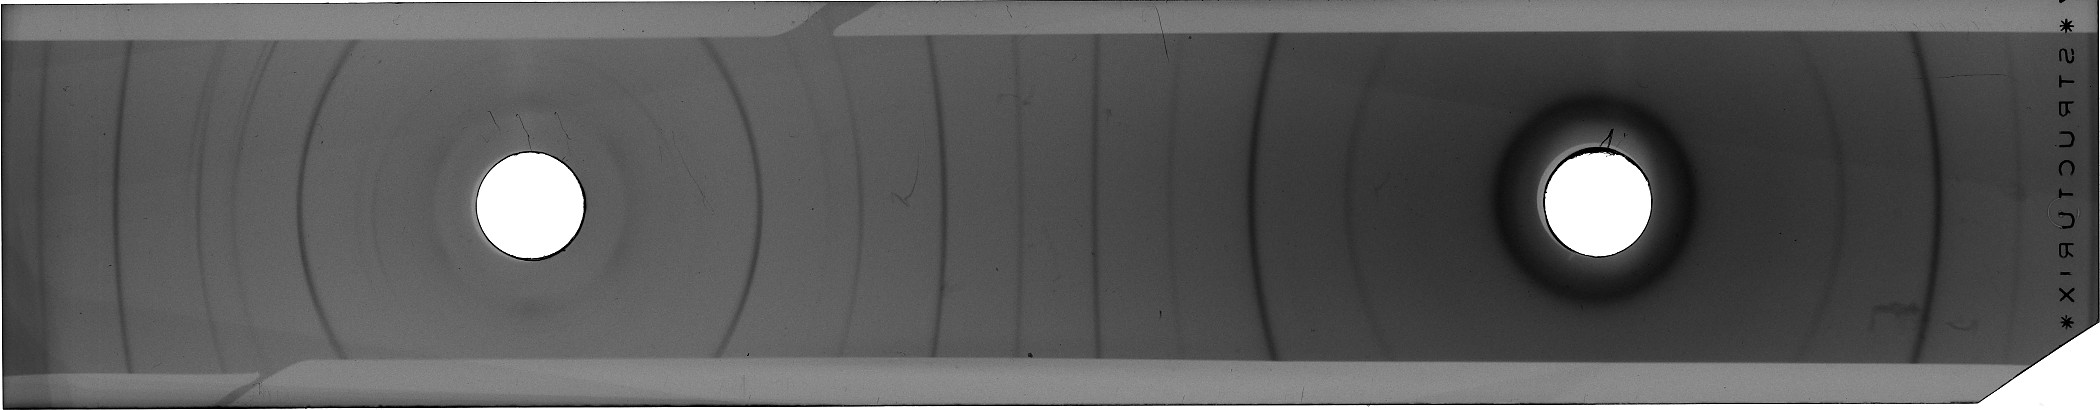
\includegraphics[width=0.9\textwidth]{Abbildungen/Roentgenfilm_Metalldraht_Filter.jpg}
    \caption{Eingescannter Röntgenfilm der Aufnahme des Metalldrahtes mit Verwendung eines Nickelfilters.}
    \label{fig:Metalldraht}
\end{figure}\\
Die Auswertung der Reflexe erfolgte analog zu der zuvor ausgewerteten Salzprobe. Für die ersten gemessenen Reflexe wurde keine passende Indizierung gefunden, allerdings war die Intensität im Vergleich zu den restlichen Reflexen sehr schwach. Da durch den Filter die schwache $K_\beta$-Linie herausgefiltert wird und keine Unterscheidung zwischen $K_{\alpha_1}$- und $K_{\alpha_2}$-Linie möglich ist, wird wieder die gemittelte Wellenlänge aus~\eqref{eqn:Wellenlänge} verwendet.
\begin{table}[ht]
	\centering
	\caption{Berechnung der Gitterkonstante des Metalldrahtes. Da die Intensität der ersten Reflexe sehr schwach war, werden diese aus der Berechnung herausgenommen.}
	\label{tab:Ergebnisse_Metalldraht}
	\begin{tabular}{l c c c c c | c c c c c}
		\toprule
      Nr. & $s [\text{inch}]$ & Intensität & $\vartheta [\si{\degree}]$ & $\Delta \vartheta [\si{\degree}]$ & $\sin^2 \vartheta $ & $Q$ & $(hkl)$ & $n$ & $a_0 [\si{\textup{\AA}}]$ & $\Delta a_0 [\si{\textup{\AA}}]$\\
    \midrule
    1  & 0,65 & sehr hell    & 8,2  & 0,3 & 0,0205 &         &     &    &        &        \\
    2  & 1,01 & sehr hell    & 12,8 & 0,2 & 0,0491 &         &     &    &        &        \\
    3  & 1,15 & sehr hell    & 14,6 & 0,1 & 0,0636 &         &     &    &        &        \\
    4  & 1,53 & dunkel       & 19,4 & 0,2 & 0,1102 & 0,05510 & 110 & 2  & 3,2835 & 0,0386 \\
    5  & 1,98 & hell         & 25,1 & 0,2 & 0,1798 &         &     &    &        &        \\
    6  & 2,21 & mitteldunkel & 28,0 & 0,3 & 0,2205 & 0,05512 & 200 & 4  & 3,2830 & 0,0401 \\
    7  & 2,76 & dunkel       & 35,0 & 0,2 & 0,3286 & 0,05476 & 211 & 6  & 3,2936 & 0,0298 \\
    8  & 3,27 & dunkel       & 41,4 & 0,3 & 0,4380 & 0,05475 & 220 & 8  & 3,2941 & 0,0339 \\
    9  & 4,27 & hell         & 54,1 & 0,4 & 0,6568 & 0,05473 & 222 & 12 & 3,2946 & 0,0344 \\
    10 & 4,81 & dunkel       & 61,0 & 0,3 & 0,7647 & 0,05462 & 321 & 14 & 3,2980 & 0,0267 \\
    11 & 5,44 & hell         & 69,0 & 0,3 & 0,8712 & 0,05445 & 400 & 16 & 3,3032 & 0,0267 \\
    12 & 6,46 & dunkel       & 81,9 & 0,5 & 0,9801 & 0.05445 & 411 & 18 & 3,3031 & 0,0378
	\end{tabular}
\end{table}\\
Die ersten vermessenen Reflexe erscheinen im Vergleich sehr schwach und liefern bei der Auswertung keine passenden Indizierungen. Die gefundenen Indizierungen zeigen, dass die Summe der $(hkl)$ stets gerade ist, was auf ein kubisch innenzentriertes Gitter hindeutet. Der letzte Reflex liefert eine Gitterkonstante von
\begin{align}
  a_0 = \SI{3,3031 \pm0,0378}{\textup{\AA}}.\label{eqn:Gitterkonstante_Metalldraht}
\end{align}
Es werden hier drei signifikante Stellen angegeben, da der berechnete Fehler für die Gitterkonstante sehr groß ist.
Zusätzlich wird wieder die \textsc{Nelson-Niley}-Extrapolation zur Bestimmung der Gitterkonstanten $a_0$ bei $\vartheta = \SI{90}{\degree}$ verwendet. Dabei ergibt sich die in Abbildung~\ref{fig:Extrapolation_Metalldraht} dargestellte lineare Funktion.
\begin{figure}[htp]
    \centering
        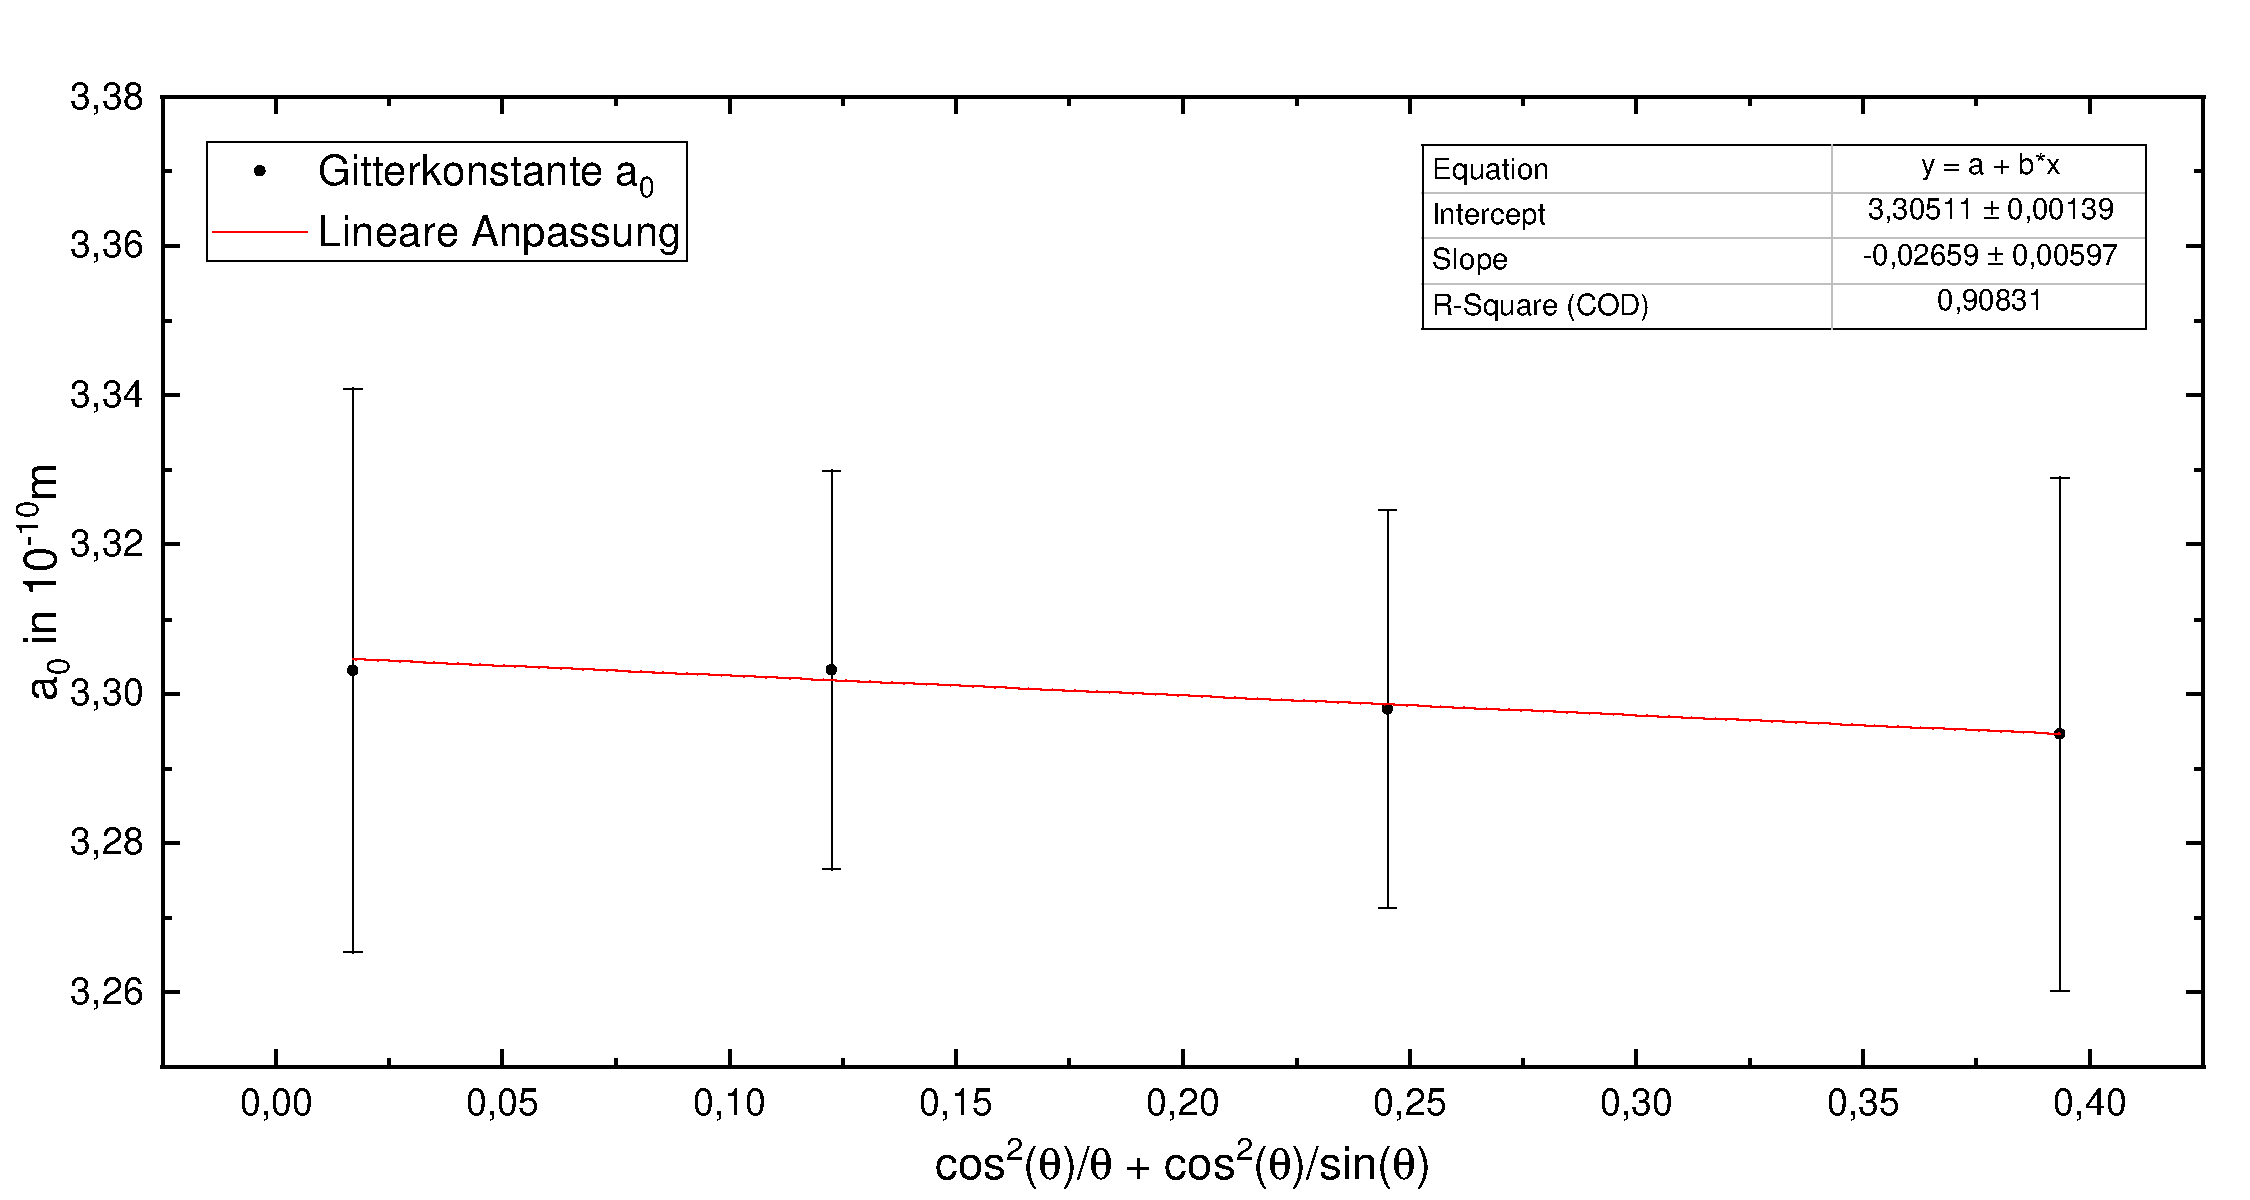
\includegraphics[width=0.9\textwidth]{Abbildungen/Extrapolation_Metalldraht.pdf}
    \caption{Extrapolationsverfahren zur Bestimmung der Gitterkonstante bei $\vartheta = \SI{90}{\degree}$.}
    \label{fig:Extrapolation_Metalldraht}
\end{figure}\\
Durch die Extrapolation ergibt sich eine Gitterkonstante von
\begin{align}
  a_0 =  \SI{3,3051 \pm 0,0060}{\textup{\AA}}.\label{eqn:Extrapolation_Metalldraht}
\end{align}
Die im Anhang von \cite{Uschmann} angegeben Gitterkonstanten zeigen eine große Übereinstimmung mit Tantal, für welches ein Literaturwert von $a_0 = \SI{3,303}{\textup{\AA}}$ angegeben wird, welcher mit~\eqref{eqn:Gitterkonstante_Metalldraht} übereinstimmt und bei~\eqref{eqn:Extrapolation_Metalldraht} im Fehlerintervall liegt. Es bestätigt ebenfalls die bestimmte Art des Gitters, denn Tantal hat einen kubisch innenzentrierten Gittertyp.

\subsection{Wertung des Debye-Scherrer-Verfahrens}
Mit dem getesteten Röntgen-Analyse-Verfahren nach Debye-Scherrer konnten die Gitterkonstanten der unterschiedlichen Stoffe genau bestimmt und die jeweiligen Stoffe sehr sicher zugeordnet werden. Außerdem ist das Messverfahren bzw. die Justage einfach und systematische Messfehler können gut korigiert werden. Als weiterer großer Vorteil ist zu sehen, dass nur pulverisiertes Material und keine größeren, gut ausgebildeten Kristalle nötig sind.\\
Schwierigkeiten und Potential für Unsicherheiten bietet das Indizieren der Reflexe, was hauptsächlich durch Ausprobieren möglich war. Außerdem können nur einfache Kristallstrukturen derart unaufwändig ausgewertet werden.


% *********************************************
% ***** KAPITEL 4 *****************************
% *********************************************
\section{Zusammenfassung}
Lorem ipsum dolor sit amet, consetetur sadipscing elitr, sed diam nonumy eirmod tempor invidunt ut labore et dolore magna aliquyam erat, sed diam voluptua. At vero eos et accusam et justo duo dolores et ea rebum. Stet clita kasd gubergren, no sea takimata sanctus est Lorem ipsum dolor sit amet. Lorem ipsum dolor sit amet, consetetur sadipscing elitr, sed diam nonumy eirmod tempor invidunt ut labore et dolore magna aliquyam erat, sed diam voluptua. At vero eos et accusam et justo duo dolores et ea rebum. Stet clita kasd gubergren, no sea takimata sanctus est Lorem ipsum dolor sit amet.

% ***** Literaturverzeichnis ******************

\begin{thebibliography}{xxx}
	\bibitem{Demtroeder}
	W. Demtröder: \textit{Experimentalphysik}. Springer Verlag Berlin Heidelberg New York 2008 (5. Auflage).
	\bibitem{Glockner}
	R. Glocker: \textit{Materialprüfung mit Röntgenstrahlen}. Springer Verlag Berlin Heidelberg New York 1985.
  \bibitem{Kleber}
	W. Kleber u.a.: \textit{Einführung in die Kristallographie}. Oldenbourg Wissenschaftsverlag 2010 (19. Auflage).
  \bibitem{Roentgenroehre}
  Aufbau einer Röntgenröhre: \url{wikimedia.org/wiki/File:WaterCooledXrayTube.svg}. Stand: 20.10.2019
  \bibitem{Uschmann}
  I.Uschmann: \textit{FSU Fortgeschrittenenen Praktikum: Debye-Scherrer-Verfahren DS}Friedrich Schiller Universität Oktober 2013
\end{thebibliography}

\end{document}
